\documentclass{article}

\usepackage{svg}
\usepackage{microtype}
\usepackage[framemethod=tikz]{mdframed}
\usepackage{hyperref}
\usepackage{url}
\usepackage{xspace}
\hypersetup{
    colorlinks,
    citecolor=black,
    filecolor=black,
    linkcolor=black,
    urlcolor=black
}

\author{Zanella Mioso}

\title{Documentazione progetto Ingegneria del Software}

\begin{document}

\maketitle

\newpage

\tableofcontents

\newpage

\section{Requisiti ed interazioni utente-sistema}

\subsection{Specifiche casi d’uso}

Il sistema è diviso in due parti principali. Una dedicata all'utente e l'altra
al responsabile del reparto. Per \textbf{utente} si intende la persona che utente questo
servizio per fare la spesa e per \textbf{responsabile reparto} l'impiegato che gestisce
il reparto a lui assegnato. L’utente non necessita di autenticarsi per consultare il
catalogo dei prodotti, ma per acquistarli deve registrarsi nel sistema, invece il
responsabile deve autenticarsi con delle credenziali pre-fortine dagli amministratori
del sistema.

\subsubsection{Casi d'uso relativi all'utente}

\begin{figure}[h!]
	\centering
	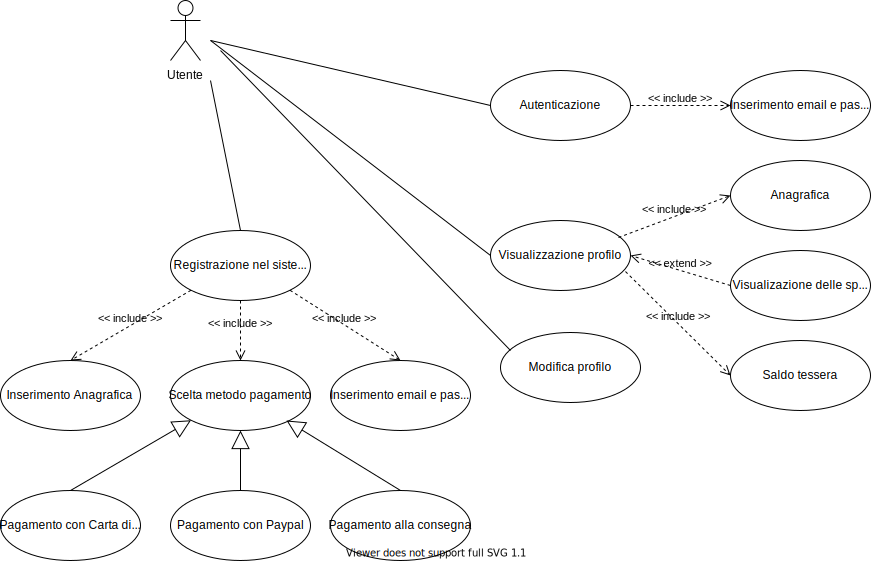
\includegraphics[width=\textwidth]{UseCaseUtenteGestioneProfilo.jpg}
	\caption{Use case di utente per la gestione del profilo e la registrazione}
	\label{fig:UseCaseUtenteGestioneProfilo}
\end{figure}

\newpage


\paragraph{Registrazione nel sistema:}

\begin{mdframed}

	\noindent\textit{\textbf{Attori :}}


	Utente

	\noindent\textit{\textbf{Descrizione :}}


	Procedura di inserimento dei dati dell’utente per registrarsi nel
	sistema

	\noindent\textit{\textbf{Sequenza di eventi :}}


	L’utente inserisce i suoi dati relativi all'anagrafica,
	scelta di metodo di pagamento preferito, email e password.

	\noindent\textit{\textbf{Post condizioni:}}


	Il sistema registra l’utente con i dati inseriti

	\noindent\textit{\textbf{Sequenza Alternativa :}}


	Se i dati inseriti non sono validi il sistema non effettua la
	registrazione
	Se l'email è già stata inserita nel sistema,
	il sistema ne richiede una diversa
\end{mdframed}

\begin{figure}[h!]
	\centering
	\includegraphics[width=\textwidth]{SDregistrazione.jpg}
	\caption{Sequence Diagram della registrazione}
	\label{fig:SDregistrazione}
\end{figure}
\newpage
\paragraph{Autenticazione:}
\begin{mdframed}

	\noindent\textit{\textbf{Attori :}}


	Utente

	\noindent\textit{\textbf{Descrizione :}}


	Procedura di autenticazione dell'utente

	\noindent\textit{\textbf{Sequenza di eventi :}}


	L’utente inserisce i dati necessari per l'autenticazione

	\noindent\textit{\textbf{Pre-condizioni:}}


	l'utente deve essere registrato nel sistema

	\noindent\textit{\textbf{Sequenza Alternativa :}}


	Se i dati inseriti non sono validi il sistema non effettua
	l'autenticazione

\end{mdframed}

\begin{figure}[h!]
	\centering
	\includegraphics[width=\textwidth]{SDautenticazione.jpg}
	\caption{Sequence Diagram dell'autenticazione}
	\label{fig:SDautenticazione}
\end{figure}

\newpage

\paragraph{Visualizzazione catalogo:}

\begin{mdframed}
	\noindent\textit{\textbf{Attori :}}


	Utente

	\noindent\textit{\textbf{Descrizione :}}


	Il sistema permette di visualizzare tutti i prodotti disponibili, e ordinarli:
	\begin{enumerate}
		\item in modo crescente e decrescente per prezzo
		\item in ordine alfabetico per marca
	\end{enumerate}

	\noindent\textit{\textbf{Sequenza di eventi :}}


	L’utente accede all'area dedicata

\end{mdframed}

\paragraph{Gestione profilo:}

\begin{mdframed}
	\noindent\textit{\textbf{Attori:}}


	Utente


	\noindent\textit{\textbf{Scopo e Descrizione sintetica:}}


	Il sistema permette all’utente di gestire il proprio profilo.
	L’utente può visualizzare e modificare il proprio profilo.

	\noindent\textit{\textbf{Sequenza di eventi :}}

	Questo caso d’uso viene attivato quando l’utente vuole modificare o visualizzare il proprio profilo.
	\begin{enumerate}
		\item L’utente sceglie la funzione richiesta
		\item Uno dei seguenti casi d’uso viene utilizzato:
		      \begin{enumerate}
			      \item{ Modifica profilo:
			            comprende la modifica dell'anagrafica.}
			      \item{Visualizzazione profilo: comprende la visualizzazione\\dell'anagrafica,
			            delle spese effettuate e l'attuale saldo punti della tessera.}
		      \end{enumerate}
	\end{enumerate}

	\noindent\textit{\textbf{Pre condizioni:}}


	L’utente deve essere registrato ed aver fatto il login 	nel sistema

	\noindent\textit{\textbf{Post-condizioni:}}


	Se le operazioni di modifica vanno a buon fine lo stato del profilo viene modificato,
	altrimenti il profilo rimane invariato.

	\noindent\textit{\textbf{Sequenza Alternativa:}}


	Se i dati inseriti non sono validi il sistema non effettua modifiche.
\end{mdframed}
\newpage

\subsubsection{Gestione carrello:}

\begin{figure}[h!]
	\centering
	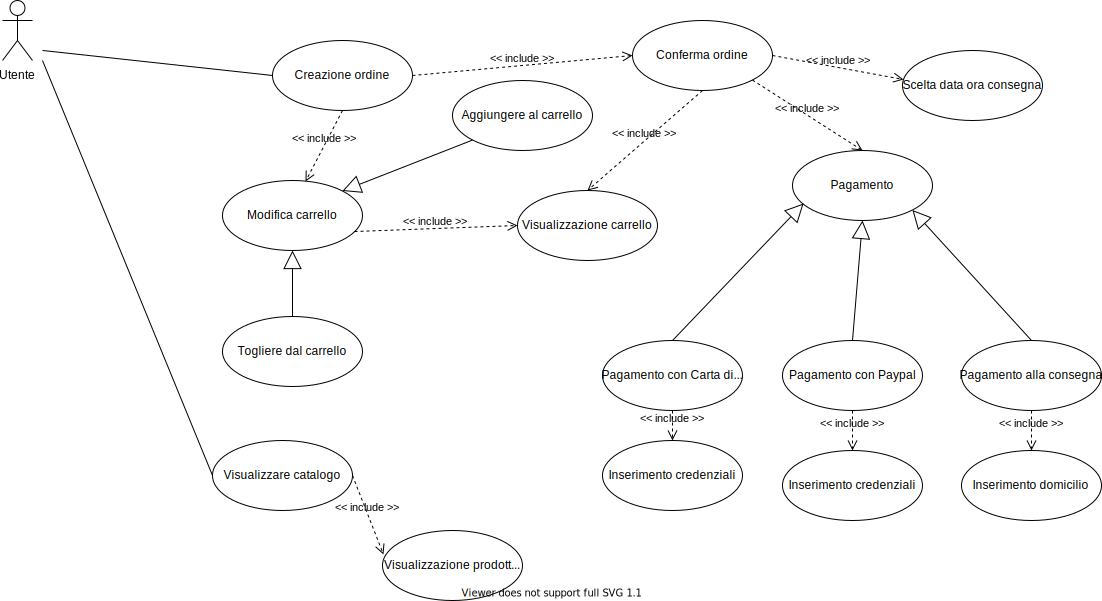
\includegraphics[width=\textwidth]{UseCaseUtenteGestioneCarrello.jpg}
	\caption{Use case del carrello}
	\label{fig:UseCaseUtenteGestioneCarrello}
\end{figure}

\newpage
\begin{mdframed}

	\noindent\textit{\textbf{Attori :}}


	Utente

	\noindent\textit{\textbf{Scopo e Descrizione sintetica :}}


	Il sistema permette all’utente di gestire il proprio carrello della spesa.
	L’utente può visualizzare il proprio carrello,
	inserire prodotti e togliere i prodotti già inseriti, confermare l’ordine e
	specificare una modalità di pagamento

	\noindent\textit{\textbf{Sequenza di eventi :}}


	\hspace{\parindent} Questo caso d’uso viene attivato quando l’utente vuole modificare il proprio carrello.
	\begin{enumerate}
		\item L’utente sceglie la funzione richiesta
		\item Uno dei seguenti casi d’uso viene utilizzato:
		      \begin{enumerate}
			      \item Modifica al carrello(aggiungere e togliere prodotti)
			      \item Visualizzazione carrello
			      \item Conferma ordine:
			            comprende la scelta di un metodo di pagamento
			            (carta di credito, paypal, consegna a domicilio)
			            inserendo per ciascuno le credenziali e il domicilio.
			            Infine viene richiesta la data e l'ora di consegna della spesa.
		      \end{enumerate}
	\end{enumerate}

	\noindent\textit{\textbf{Pre condizioni:}}


	L’utente deve essere registrato ed aver fatto il login 	nel sistema

	\noindent\textit{\textbf{Post-condizioni:}}


	Se le operazioni di modifica vanno a buon fine lo stato del carrello viene modificato,
	altrimenti il contenuto del carrello rimane invariato.
	Se il pagamento va a buon fine l’acquisto viene fatto, altrimenti l’acquisto
	non viene effettuato.

	\noindent\textit{\textbf{Sequenza Alternativa :}}


	Se durante la conferma il prodotto non è disponibile, viene visualizzato un
	messaggio di errore per informare l’utente che il prodotto non è disponibile.
	Se i dati inseriti non sono validi il sistema non effettua modifiche.
\end{mdframed}
\newpage
\begin{figure}[h!]
	\centering
	\includegraphics[width=\textwidth]{SDGestioneCarrello.jpg}
	\caption{Sequence Diagramm della gestione del carrello}
	\label{fig:SDGestioneCarrello}
\end{figure}

\begin{figure}[h!]
	\centering
	\includegraphics[width=\textwidth]{SDConfermaOrdine.jpg}
	\caption{Sequence Diagramm della conferma dell'ordine}
	\label{fig:SDConfermaOrdine}
\end{figure}
\newpage
\clearpage
\subsubsection{Casi d'uso relativi al responsabile reparto}

\begin{figure}[h!]
	\centering
	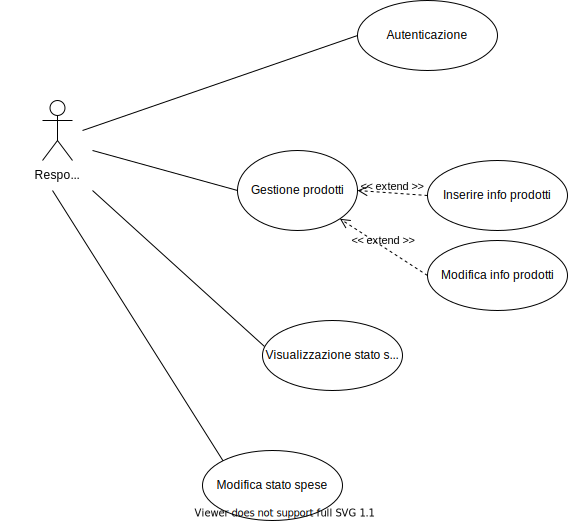
\includegraphics[width=\textwidth]{UseCaseResponsabile.jpg}
	\caption{Use case di responsabile reparto per l'autenticazione la gestione delle spese e dei prodotti}
	\label{fig:UseCaseResponsabile}
\end{figure}

\paragraph{Autenticazione:}
\begin{mdframed}

	\noindent\textit{\textbf{Attori :}}


	Responsabile reparto

	\noindent\textit{\textbf{Descrizione :}}


	Procedura di autenticazione del responsabile di reparto

	\noindent\textit{\textbf{Sequenza di eventi :}}


	Il responsabile inserisce i dati necessari per l'autenticazione

	\noindent\textit{\textbf{Pre-condizioni:}}


	Il responsabile deve essere presente nel sistema

	\noindent\textit{\textbf{Sequenza Alternativa :}}


	Se i dati inseriti non sono validi il sistema non effettua
	l'autenticazione

\end{mdframed}

\paragraph{Visualizzazione stato spese:}
\begin{mdframed}

	\noindent\textit{\textbf{Attori :}}


	Responsabile reparto

	\noindent\textit{\textbf{Descrizione :}}


	Sono visualizzati i dati relativi alle spese dei clienti.

	\noindent\textit{\textbf{Sequenza di eventi :}}


	Il responsabile accede all'area dedicata

	\noindent\textit{\textbf{Pre-condizioni:}}


	Il responsabile di reparto aver fatto il login nel sistema


	\noindent\textit{\textbf{Sequenza alternativa:}}


	Se i dati inseriti non sono validi il sistema non effettua modifiche

\end{mdframed}

\paragraph{Gestione prodotti}

\begin{mdframed}

	\noindent\textit{\textbf{Attori :}}


	Responsabile reparto

	\noindent\textit{\textbf{Descrizione :}}


	Il sistema permette al responsabile di gestire i prodotti del proprio reparto
	Con la possibilità di modificare e aggiungere i prodotti che sono terminati o che stanno
	per terminare.
	Inotre può inserire nel sistema nuovi prodotti che appariranno sul catalogo

	\noindent\textit{\textbf{Sequenza di eventi :}}


	Il responsabile accede all'area dedicata

	\noindent\textit{\textbf{Pre-condizioni:}}


	Il responsabile di reparto aver fatto il login nel sistema

	\noindent\textit{\textbf{Sequenza alternativa:}}


	Se i dati inseriti non sono validi il sistema non effettua modifiche
\end{mdframed}


\section{Sviluppo: progetto dell'architettura ed implemtazione del sistema}
\subsection{Note sul processo di sviluppo}
\subsection{Progettazione e pattern architetturali usati}
\subsubsection{Pattern MVC}
Il progetto è strutturato con il Pattern MVC, perché fornisce una coerenza strutturale solida 
semplificando le fasi di progettazione e implementazione. Inoltre crea un'ottima sinergia con la
piattaforma JavaFX.


Il sistema è suddiviso in tre parti:
\begin{itemize}
    \item{\textbf{Model:}
            Sono presenti le classi che definiscono i dati manipolati
            Inoltre sono presenti le classi che permettono la comunicazione
            con il Database organizzate seguendo il DAO pattern.
        }
    \item{\textbf{View:}
            Parte esclusivamente dedicata alla visualizzazione dei dati
            presenti nel modello.
            In particolare si utilizzano file .fxml
        }
    \item{\textbf Controller:}
\end{itemize}
\subsection{Note su JavaFX}
\subsection{Implementazione e desing pattern usati}
\subsubsection{Pattern Sigleton}
\subsubsection{Pattern Observer}
\subsubsection{Pattern Data Access Object}
\subsubsection{UML delle Classi}
\begin{figure}[h!]
	\centering
	\includegraphics[width=\textwidth]{UmlProdotto.png}
	\caption{UML della classe Prodotto}
	\label{fig:UmlProdotto}
\end{figure}

\begin{figure}[h!]
	\centering
	\includegraphics[width=\textwidth]{UmlSpesa.png}
	\caption{UML della classe Spesa e Carrello in relazione con Prodotto}
	\label{fig:UmlSpesa}
\end{figure}


\begin{figure}[h!]
	\centering
	\includegraphics[width=\textwidth]{UmlCatalog.jpg}
	\caption{UML delle classi dell vista Catalogo}
	\label{fig:UmlCatalog}
\end{figure}

\begin{figure}[h!]
	\centering
	\includegraphics[width=\textwidth]{UmlInterfaccie.jpg}
	\caption{UML delle Classi di tutte le viste}
	\label{fig:UmlInterfaccie}
\end{figure}

\clearpage
\subsection{Persistenza dati con Database SQL}
\subsubsection{Diagramma ER}

\begin{figure}[h!]
	\centering
	\includegraphics[width=\textwidth]{DiagrammaER.png}
	\caption{Diagramma Entity Relationship}
	\label{fig:DiagrammaER}
\end{figure}

\end{document}
